% !TEX TS-program = pdflatexmk
\documentclass[12pt]{article}

% Layout.
\usepackage[top=1in, bottom=0.75in, left=1in, right=1in, headheight=1in, headsep=6pt]{geometry}

% Fonts.
\usepackage{mathptmx}
\usepackage[scaled=0.86]{helvet}
\renewcommand{\emph}[1]{\textsf{\textbf{#1}}}

% TiKZ.
\usepackage{tikz, pgfplots}
\usetikzlibrary{calc}
\pgfplotsset{my style/.append style={axis x line=middle, axis y line=
middle, xlabel={$x$}, ylabel={$y$}, axis equal }}

% Misc packages.
\usepackage{amsmath,amssymb,latexsym}
\usepackage{graphicx}
\usepackage{array}
\usepackage{xcolor}
\usepackage{multicol}

% Commands to set various header/footer components.
\makeatletter
\def\doctitle#1{\gdef\@doctitle{#1}}
\doctitle{Use {\tt\textbackslash doctitle\{MY LABEL\}}.}
\def\docdate#1{\gdef\@docdate{#1}}
\docdate{Use {\tt\textbackslash docdate\{MY DATE\}}.}
\def\doccourse#1{\gdef\@doccourse{#1}}
\let\@doccourse\@empty
\def\docscoring#1{\gdef\@docscoring{#1}}
\let\@docscoring\@empty
\def\docversion#1{\gdef\@docversion{#1}}
\let\@docversion\@empty
\makeatother

% Headers and footers layout.
\makeatletter
\usepackage{fancyhdr}
\pagestyle{fancy}
\fancyhf{} % Clears all headers/footers.
\lhead{\baselineskip 30pt
\emph{\@doctitle\hfill\@docdate}
\ifnum \value{page} > 1\relax\else\\
\emph{Name: \rule{3.5in}{1pt}\hfill \@docscoring}\fi}
\rfoot{\emph{\@docversion}}
\lfoot{\emph{\@doccourse}}
\cfoot{\emph{\thepage}}
\renewcommand{\headrulewidth}{0pt}%
\makeatother

% Paragraph spacing
\parindent 0pt
\parskip 6pt plus 1pt

% A problem is a section-like command. Use \problem{5} to
% start a problem worth 5 points.
\newcounter{probcount}
\newcounter{subprobcount}
\setcounter{probcount}{0}
\newcommand{\problem}[1]{%
\par
\addvspace{4pt}%
\setcounter{subprobcount}{0}%
\stepcounter{probcount}%
\makebox[0pt][r]{\emph{\arabic{probcount}.}\hskip1ex}\emph{[#1 points]}\hskip1ex}
\newcommand{\thesubproblem}{\emph{\alph{subprobcount}.}}

% Subproblems are an enumerate-like environment with a consistent
% numbering scheme. 
% Use \begin{subproblems}\item...\item...\end{subproblems}
\newenvironment{subproblems}{%
\begin{enumerate}%
\setcounter{enumi}{\value{subprobcount}}%
\renewcommand{\theenumi}{\emph{\alph{enumi}}}}%
{\setcounter{subprobcount}{\value{enumi}}\end{enumerate}}

% Blanks for answers in normal and math mode.
\newcommand{\blank}[1]{\rule{#1}{0.75pt}}
\newcommand{\mblank}[1]{\underline{\hspace{#1}}}
\def\emptybox(#1,#2){\framebox{\parbox[c][#2]{#1}{\rule{0pt}{0pt}}}}

% Misc.
\renewcommand{\d}{\displaystyle}
\newcommand{\ds}{\displaystyle}
\def\bc{\begin{center}}
\def\ec{\end{center}}


\doctitle{Math 251: Quiz 3}
\docdate{September 17, 2019}
\doccourse{UAF Calculus I}
\docversion{v-1}
\docscoring{\blank{0.8in} / 25}
\begin{document}
There are 25 points possible on this quiz. No aids (book, calculator, etc.)
are permitted.  Show all work for full credit.

\problem{2} Use the graph of the function of $f(x)$ to find \emph{all} $x$-values where $f(x)$ fails to be continuous.\\
%\begin{center}
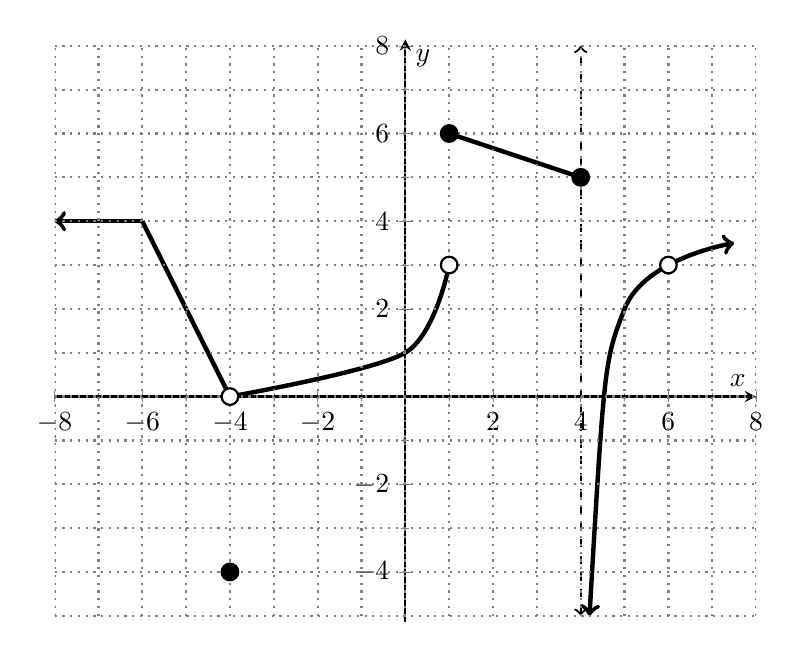
\begin{tikzpicture}
\begin{axis}[scale=1.3, thick, my style, xtick={-8,-6,...,8}, ytick={-4,-2,...,8},
xmin=-8, xmax=8, ymin=-5, ymax=8, minor y tick num=1,
        minor x tick num=1, mark size=3.0pt]
 %%asymptote
\addplot[dashed,<->, thick] coordinates {(4,-5) (4,8)};
%points solid
\addplot[mark=*,only marks] coordinates {(-4,-4)(4,5)(1,6)};
%points open
\addplot[mark=*,fill=white,only marks] coordinates {(-4,0)
(1,3) (6,3)};
\addplot[ultra thick, smooth,->] coordinates {(-6,4) (-8,4)};
\addplot[ultra thick, smooth] coordinates {(-4,0) (-6,4)};
\addplot[ultra thick, smooth,] coordinates {(-4,0) (0,1) (1,3)};
\addplot[ultra thick, smooth] coordinates {(1,6)(4,5)};
\addplot[ultra thick, smooth,<->] coordinates {(4.2,-5) (5,2) (7.5,3.5)};
\foreach \i in {-8,-7,-6,...,8}{
	\addplot[dotted, gray, domain=-8:8]{\i};
	\addplot[dotted, gray] coordinates {(\i,-5) (\i,8)};
	}
\end{axis}
\end{tikzpicture}
%\end{center}
\hfill
\textbf{Answer: $x = $\underline{\hspace{1.5in}}}



\problem{4}\begin{subproblems}
\item
What is wrong with the following equation?\qquad $\ds \frac{x-4x^3}{x} = 1-4x^2$
\vskip 0.75in

\item 
In view of part a, explain why the following equation is correct.\qquad
$\ds
\lim_{x\to0}\frac{x-4x^3}{x} = \lim_{x\to0}1-x^2
$
\vskip 0.75in
\end{subproblems}



\problem{4} Explain why the function 
$\ds
f(x)=\begin{cases} 4\sin x & x < 0\\ 0 & x=0\\
4x-2 & x>0.
\end{cases}
$
fails to be continuous at $x=0.$
\vfill
%\begin{subproblems}
%\item In the diagram below, graph $f(x)$.
%\begin{center}
%\begin{tikzpicture}[scale=1.0]
%\draw [help lines,dashed] (-6.2,-3.2) grid (6.2,3.2);
%
%\draw [thick, ->] (-6.2,0)--(6.2,0) node[right] {$x$};
%\draw [thick, ->] (0,-3.2)--(0,3.2) node[above]{$f(x)$};
%
%\foreach \i in {-4,-2,2,4}
%{	\node[below] at (\i,0) {$\i$};
%}
%\foreach \i in {-2,2}
%{	\node[left] at (0,\i) {$\i$};
%}
%\end{tikzpicture}
%\end{center}

%\item Explain why $f(x)$ isn't continuous at $x=0$.
%\end{subproblems}
%\vskip 2cm

%\problem{4} Use the Intermediate Value Theorem to justify the
%claim that there exists a number $x$ satisfying
%$\ds 2^x-x-4 = 0.$
\newpage
\problem{12} Evaluate each limit below, if it exists. Show your work to receive full credit. If the limit is infinite, say so; don't just write ``DNE".
\begin{subproblems}
\item  $\ds \lim_{x\to 2}\frac{x^2+5x-14}{2+x-x^2}$.
\vfill

\item $\ds \lim_{h\to 10^-}\frac{ 2|h|-20}{h-10}$
\vfill

\item  $\ds \lim_{x\to 5^+} \left(\frac{ 1}{x-5}-\frac{1}{x(x-5)}\right)$
\vfill
\end{subproblems}

\problem{3} What property of the square root function allows you to move the limit inside the square root, as done below.

$$\lim_{x \to 5} \sqrt{x^2+9} = \sqrt{\lim_{x \to 5} (x^2+9)}$$

\vfill
\end{document}